\documentclass[../ClipsManualeUtente.tex]{subfiles}

\begin{document}
\section{Installazione}
	Di seguito si elencano i passaggi necessari per la corretta installazione dell'applicazione nello smartphone.
	
		\subsection{Disattivare i controlli di sicurezza}
			???

		\subsection{Download e installazione applicazione}		
		\begin{enumerate}
			\item dal proprio smartphone aprire il browser preferito;
			\item digitare correttamente il seguente indirizzo web: \\
				\url{http://leafswe.github.io/download/}
			\item premere il pulsante \textbf{download} come in figura \ref{fig:DownloadApplicazioneSito};
			\item accettare il download;
			\item selezionare il file \lstinline|clips.apk| scaricato;
			\item accettare che l'applicazione sia installata nel proprio dispositivo.
		\end{enumerate}
		
		\begin{figure} [h]
			\centering
			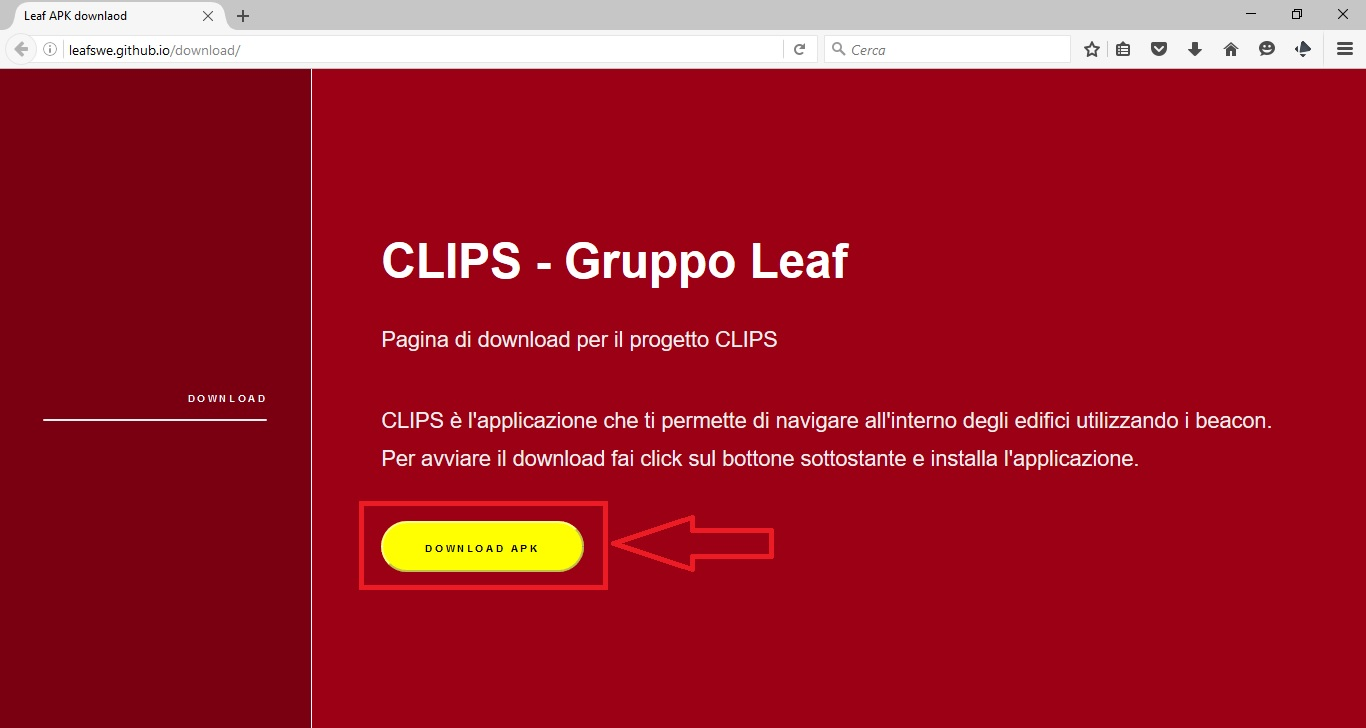
\includegraphics[width=\textwidth]{img/DownloadApplicazioneSito}
			\caption{Pagina del sito da cui effettuare il download dell'applicazione}
			\label{fig:DownloadApplicazioneSito}
		\end{figure}
		
\end{document}